\clearpage
\subsection{Global Variable} % (fold)
\label{sub:global_variable}

Variables and Constants can be declared within a Program. Variables declared in this way are called Global Variables. It seems tempting to use Global Variables to share values between procedures, but this is a bad idea. Global Variables should be avoided, and for many programs are unnecessary. The issue with Global Variables is that their values can be changed from anywhere within the program's code. This can make it difficult to locate the source of errors when globals are used.

While Global Variables should be avoided, Constants should be declared globally. As these values can not change, the issues with Global Variables do not affect Constants. 

\begin{figure}[h]
   \centering
   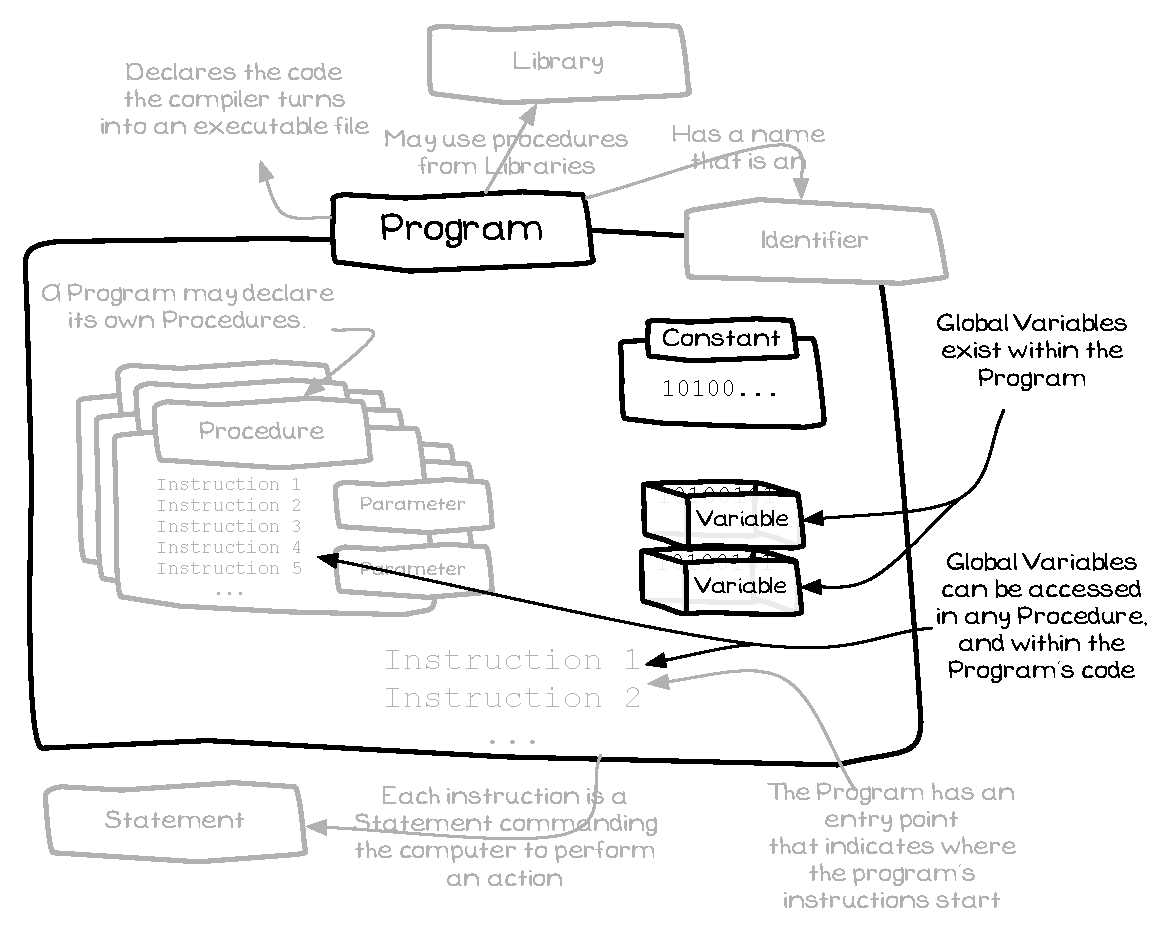
\includegraphics[width=\textwidth]{./topics/storing-using-data/diagrams/GlobalVariables} 
   \caption{Variables declared within a Program are Global Variables}
   \label{fig:storing-using-data-global-variables}
\end{figure}

\mynote{
\begin{itemize}
  \item Global Variable is the \textbf{term} given to a Variable that is declared within the program.
  \item Variables that are declared within a Program are called \textbf{Global Variables}.
  \item Global Variables can be accessed by the program's instructions, and by the instructions in any of the Procedures.
  \item You should \textbf{avoid} using Global Variables. These variables can be accessed anywhere within the Program, making it difficult to locate errors.
  \item Using Global Variables introduces hidden dependencies between Procedures, breaking the isolated nature of the Procedures.
  \item Constants \textbf{should} be declared globally, and used to give meaning to values entered into your code.
  % \item \emph{Magic Numbers} is a term used to describe numeric Literals where the value's meaning is hard to determine. From the perspective of the reader these values are chosen by \emph{magic}. It is poor practice to have \emph{magic numbers}, and these should be replaced by Constants. For example, the value \texttt{42} may appear in code, but what does that mean? If this were called \texttt{BUTTON\_HEIGHT}, its meaning would be known.
\end{itemize}
}

% subsection global_variables (end)